% !TeX root = ../main.tex

\chapter{DPU 测试日志}

\section{2023.11.15~第一次上电}

器件采购商将 LTM4644-1 发成 LTM4644 导致 DC-DC 输出电压不对,需修改值如下:
\begin{itemize}
  \item R675: 90.9k\qquad for 1.0V
  \item R678: 30.1k\qquad for 1.8V
  \item R684: 13.3k\qquad for 3.3V
  \item R691: 10k, R690: 68k\qquad for 2.5V
  \item R699: 60.4k\qquad for 1.2V
  \item R703: 12k, R702: 20k\qquad for 1.35V
  \item R707: 5.66k, R706: 60.4k\qquad for 3.8V
  \item R711: 3.9k, R710: 68k\qquad for 5.5V
  \item R674, R677, R683, R698 去掉, (LTM4644 已内置 60.4k)
\end{itemize}

绿色LED封装画反: D1, D26, D27, D28, D29, D30, D31, D32, D33, D41, D47, D48 \par
红色LED封装画反: D40, D42 \par
FT232HL做为Xilinx的JTAG时,需要往EEPROM里烧写数据。网址: \href{https://github.com/TerayTech/TT_Digilent_JTAG_HS2}{https://github.com/TerayTech/TT\_Digilent\_JTAG\_HS2}。 烧写频率默认为15000000, 可以正常烧写程序, 烧写ILA时报错, 需把频率调为7500000。\par

\section{2023.11.18~PLL调试}

LMK04610 的一路 VCC2.5VA 未提供,从TP8测试点飞线到 C395 左侧Pin1后,LMK04610 工作正常。
%修改的寄存器表如下:
%\inputminted{shell}{./figures/pll_rom.mem} \par

\section{2023.11.20~验证时钟配置}

\section{2023.11.21~Flash配置}
逻辑无法固化,检查原理图发现,U8 Flash 的 CS 信号错接到 U34 DS18S20 的 DQ 上,将U34 去掉后,将U8 的 7脚飞到 U34 的 4脚。\par
差分LEMO连接器无法插上,把D36、D37、D38、D39去掉即可。

%\section{2023.11.26~ADC 寄存器解读\textsl{}}
%\mintinline{shell}|0a3000|: Initialization after power-up. \par
%\mintinline{shell}|000000|: Register readout disabled \& Reset disabled. \par
%\mintinline{shell}|010060|: JESD interface enabled \& LVDS interface disabled \& 32-channel input. \par

\section{2024.01.09~FPGA GT Bank供电问题}
FPGA GT Bank供电不足,导致4片ADC无法同时工作。经检查发现,电源分配中,1.8VD 同时给 1.0VA 的 FPGA 内核和 1.2VA 的FPGA GT Bank 供电,用直流电源替换 1.8VD 的供电端,显示超过 LTM4644 的最大输出电流 4A。\par
尝试解决方案:\par
如图 \ref{fig:powersolution1},在U43器件周围,沿着绿色的画线,把表层的铜皮割断;然后再沿着蓝色的画线,把它们用飞线连上。最后用飞线将 C711 右侧的 1.2VD 供电端飞到 C683 右侧的管脚上。\par
\begin{figure}[htbp]
  \centering
  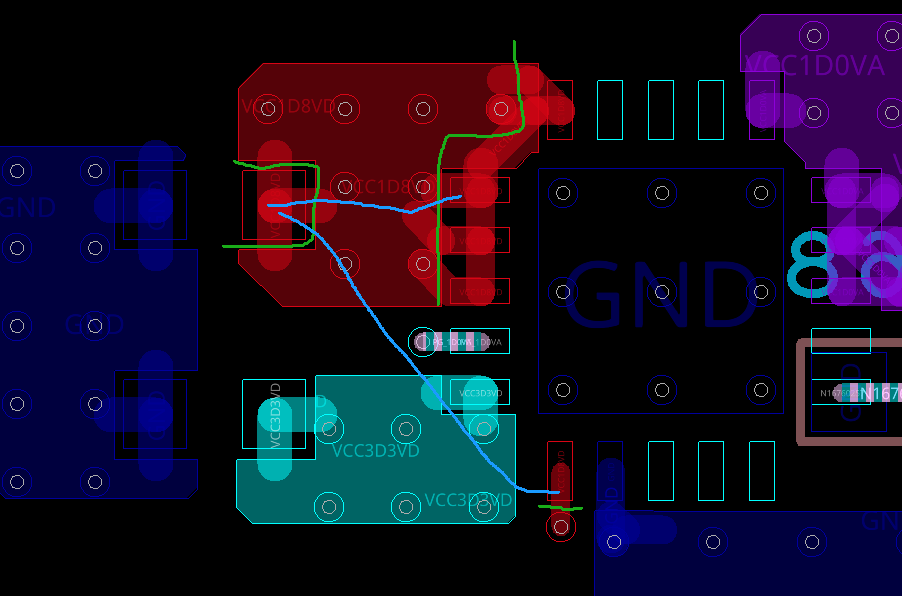
\includegraphics[width=0.65\textwidth]{powersolution1.png}
  \caption{电源解决方案1}
  \label{fig:powersolution1}
\end{figure}
来实现 FPGA 内核与 FPGA GT Bank 的分离供电。\par
为解决,仍然无法负载4个GT Bank,考虑后续改版。\par

\section{2024.01.15~FEB调试}
两块焊接完成的FEB电压测试正常,其中一块的稳压二极管不工作,更换后正常。\par
用两块ADC,连接FEB测试基线,其中有一半基线正常为设置的 \SI{-0.8}{V} 左右, 另一半基线异常为 \SI{0.8}{V} 左右,如图所示。经检查发现,FEB 中 FDA 的输出有一半接反了。\par
\begin{figure}[!htbp]
  \centering
  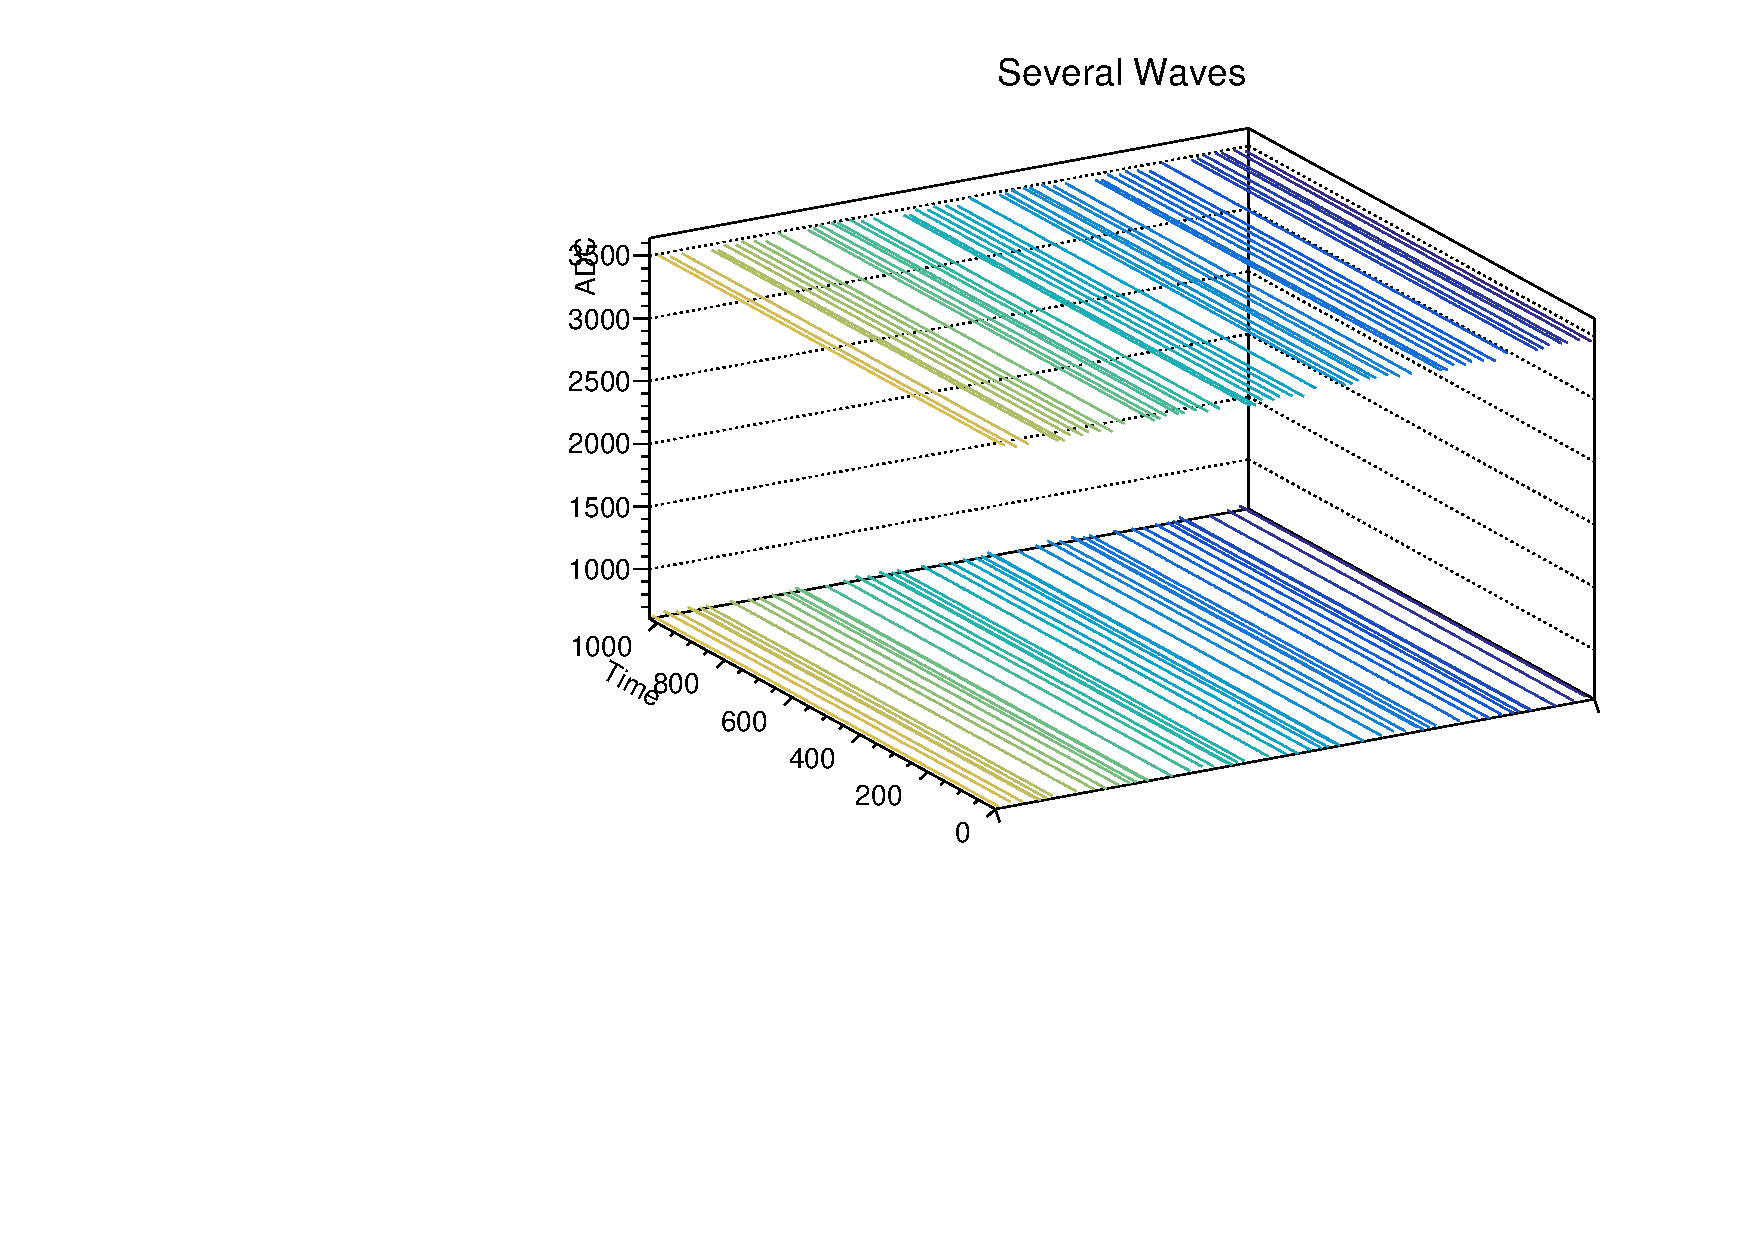
\includegraphics[width=0.85\textwidth]{240115_34_wfeb_SeveralWaves_inv.pdf}
  \caption{ADC[4:3] 连接FEB测试基线}
  \label{fig:adc34_wfeb}
\end{figure}
FEB 中 FDA 接反的通道有:1、7、69、13、3、67、23、9、79、17、85、29、81、86、25、90、95、89、27、83、31、88、21、19、74、11、70、73、15、72、65、5、39、97、104、35、99、47、41、111、55、116、49、63、125、61、59、123、127、121、57、118、113、51、120、53、43、106、45、102、105、33、101、37。\par
ADC 各通道与 TPC 阳极条对应关系如表所示:
\begin{table}[!htbp]
  \centering
  \caption{ADC 通道与 TPC 阳极条对应关系}
  \label{tab:feb_map_tpc}
  \begin{tabular}{p{0.1\textwidth}p{0.1\textwidth}p{0.1\textwidth}p{0.1\textwidth}p{0.1\textwidth}p{0.1\textwidth}p{0.1\textwidth}p{0.1\textwidth}}
  \toprule
  ADC[0] 通道号 & TPC 阳极条 & ADC[1] 通道号 & TPC 阳极条 & ADC[2] 通道号 & TPC 阳极条 & ADC[3] 通道号 & TPC 阳极条 \\
 \midrule
  %0	  & Y55 & 32  & Y21 & 64  & Y56 & 96  & Y26 \\
  %1   & X55 & 33  & X21 & 65  & X56 & 97  & X26 \\
  %2   & Y53 & 34  & Y23 & 66  & Y52 & 98  & Y22 \\
  %3   & X53 & 35  & X23 & 67  & X58 & 99  & X28 \\
  %4   & Y57 & 36  & Y27 & 68  & Y58 & 100 & Y28 \\
  %5   & X57 & 37  & X27 & 69  & Y54 & 101 & Y24 \\
  %6   & Y59 & 38  & Y25 & 70  & A4  & 102 & X30 \\
  %7   & X59 & 39  & X25 & 71  & A6  & 103 & Y30 \\
  %8   & Y47 & 40  & Y19 & 72  & A7  & 104 & Y20 \\
  %9   & X47 & 41  & X19 & 73  & Y48 & 105 & Y16 \\
  %10  & Y45 & 42  & Y9  & 74  & X48 & 106 & X16 \\
  %11  & X45 & 43  & X9  & 75  & A5  & 107 & X20 \\
  %12  & Y49 & 44  & Y17 & 76  & X52 & 108 & X22 \\
  %13  & X49 & 45  & X17 & 77  & X50 & 109 & X18 \\
  %14  & Y51 & 46  & Y15 & 78  & Y50 & 110 & Y18 \\
  %15  & X51 & 47  & X15 & 79  & X54 & 111 & X24 \\
  %16  & Y39 & 48  & Y5  & 80  & Y38 & 112 & Y6  \\
  %17  & X39 & 49  & X5  & 81  & X38 & 113 & X6  \\
  %18  & Y37 & 50  & Y7  & 82  & Y40 & 114 & X8  \\
  %19  & X37 & 51  & X7  & 83  & X44 & 115 & Y12 \\
  %20  & Y41 & 52  & Y13 & 84  & Y44 & 116 & X12 \\
  %21  & X41 & 53  & X13 & 85  & Y42 & 117 & Y10 \\
  %22  & Y43 & 54  & Y11 & 86  & X46 & 118 & X14 \\
  %23  & X43 & 55  & X11 & 87  & Y46 & 119 & Y14 \\
  %24  & Y31 & 56  & Y1  & 88  & Y32 & 120 & Y0  \\
  %25  & X31 & 57  & X1  & 89  & Y34 & 121 & X2  \\
  %26  & Y29 & 58  & Y3  & 90  & X34 & 122 & Y2  \\
  %27  & X29 & 59  & X3  & 91  & X32 & 123 & X0  \\
  %28  & Y33 & 60  & A2  & 92  & X40 & 124 & Y8  \\
  %29  & X33 & 61  & A0  & 93  & X36 & 125 & X4  \\
  %30  & Y35 & 62  & A3  & 94  & Y36 & 126 & Y4  \\
  %31  & X35 & 63  & A1  & 95  & X42 & 127 & X10 \\
  \cellcolor[HTML]{AA0044}0	  & Y55 & \cellcolor[HTML]{AA0044}32  & Y21 & \cellcolor[HTML]{AA0044}64  & Y56 & \cellcolor[HTML]{AA0044}96  & Y26 \\
  1   & X55 & 33  & X21 & 65  & X56 & 97  & X26 \\
  \cellcolor[HTML]{AA0044}2   & Y53 & \cellcolor[HTML]{AA0044}34  & Y23 & \cellcolor[HTML]{AA0044}66  & Y52 & \cellcolor[HTML]{AA0044}98  & Y22 \\
  3   & X53 & 35  & X23 & 67  & X58 & 99  & X28 \\
  \cellcolor[HTML]{AA0044}4   & Y57 & \cellcolor[HTML]{AA0044}36  & Y27 & \cellcolor[HTML]{AA0044}68  & Y58 & \cellcolor[HTML]{AA0044}100 & Y28 \\
  5   & X57 & 37  & X27 & \cellcolor[HTML]{AA0044}69  & Y54 & \cellcolor[HTML]{AA0044}101 & Y24 \\
  \cellcolor[HTML]{AA0044}6   & Y59 & \cellcolor[HTML]{AA0044}38  & Y25 & 70  & A4  & 102 & X30 \\
  7   & X59 & 39  & X25 & \cellcolor[HTML]{AA0044}71  & A6  & \cellcolor[HTML]{AA0044}103 & Y30 \\
  \cellcolor[HTML]{AA0044}8   & Y47 & \cellcolor[HTML]{AA0044}40  & Y19 & \cellcolor[HTML]{AA0044}72  & A7  & \cellcolor[HTML]{AA0044}104 & Y20 \\
  9   & X47 & 41  & X19 & \cellcolor[HTML]{AA0044}73  & Y48 & \cellcolor[HTML]{AA0044}105 & Y16 \\
  \cellcolor[HTML]{AA0044}10  & Y45 & \cellcolor[HTML]{AA0044}42  & Y9  & 74  & X48 & 106 & X16 \\
  11  & X45 & 43  & X9  & 75  & A5  & 107 & X20 \\
  \cellcolor[HTML]{AA0044}12  & Y49 & \cellcolor[HTML]{AA0044}44  & Y17 & 76  & X52 & 108 & X22 \\
  13  & X49 & 45  & X17 & 77  & X50 & 109 & X18 \\
  \cellcolor[HTML]{AA0044}14  & Y51 & \cellcolor[HTML]{AA0044}46  & Y15 & \cellcolor[HTML]{AA0044}78  & Y50 & \cellcolor[HTML]{AA0044}110 & Y18 \\
  15  & X51 & 47  & X15 & 79  & X54 & 111 & X24 \\
  \cellcolor[HTML]{AA0044}16  & Y39 & \cellcolor[HTML]{AA0044}48  & Y5  & \cellcolor[HTML]{AA0044}80  & Y38 & \cellcolor[HTML]{AA0044}112 & Y6  \\
  17  & X39 & 49  & X5  & 81  & X38 & 113 & X6  \\
  \cellcolor[HTML]{AA0044}18  & Y37 & \cellcolor[HTML]{AA0044}50  & Y7  & \cellcolor[HTML]{AA0044}82  & Y40 & 114 & X8  \\
  19  & X37 & 51  & X7  & 83  & X44 & \cellcolor[HTML]{AA0044}115 & Y12 \\
  \cellcolor[HTML]{AA0044}20  & Y41 & \cellcolor[HTML]{AA0044}52  & Y13 & \cellcolor[HTML]{AA0044}84  & Y44 & 116 & X12 \\
  21  & X41 & 53  & X13 & \cellcolor[HTML]{AA0044}85  & Y42 & \cellcolor[HTML]{AA0044}117 & Y10 \\
  \cellcolor[HTML]{AA0044}22  & Y43 & \cellcolor[HTML]{AA0044}54  & Y11 & 86  & X46 & 118 & X14 \\
  23  & X43 & 55  & X11 & \cellcolor[HTML]{AA0044}87  & Y46 & \cellcolor[HTML]{AA0044}119 & Y14 \\
  \cellcolor[HTML]{AA0044}24  & Y31 & \cellcolor[HTML]{AA0044}56  & Y1  & \cellcolor[HTML]{AA0044}88  & Y32 & \cellcolor[HTML]{AA0044}120 & Y0  \\
  25  & X31 & 57  & X1  & \cellcolor[HTML]{AA0044}89  & Y34 & 121 & X2  \\
  \cellcolor[HTML]{AA0044}26  & Y29 & \cellcolor[HTML]{AA0044}58  & Y3  & 90  & X34 & \cellcolor[HTML]{AA0044}122 & Y2  \\
  27  & X29 & 59  & X3  & 91  & X32 & 123 & X0  \\
  \cellcolor[HTML]{AA0044}28  & Y33 & \cellcolor[HTML]{AA0044}60  & A2  & 92  & X40 & \cellcolor[HTML]{AA0044}124 & Y8  \\
  29  & X33 & 61  & A0  & 93  & X36 & 125 & X4  \\
  \cellcolor[HTML]{AA0044}30  & Y35 & \cellcolor[HTML]{AA0044}62  & A3  & \cellcolor[HTML]{AA0044}94  & Y36 & \cellcolor[HTML]{AA0044}126 & Y4  \\
  31  & X35 & 63  & A1  & 95  & X42 & 127 & X10 \\
  \bottomrule
  \end{tabular}
\end{table}
修改DataAnalysis代码发现,ADC[3] 的异常通道对应ADC[2] 的异常通道,与表中查找的不一致。经修改后得到如图\ref{fig:ADC_wfeb}所示基线。\par
\begin{figure}[htbp]
  \centering
  \begin{subfigure}[b]{0.45\textwidth}
    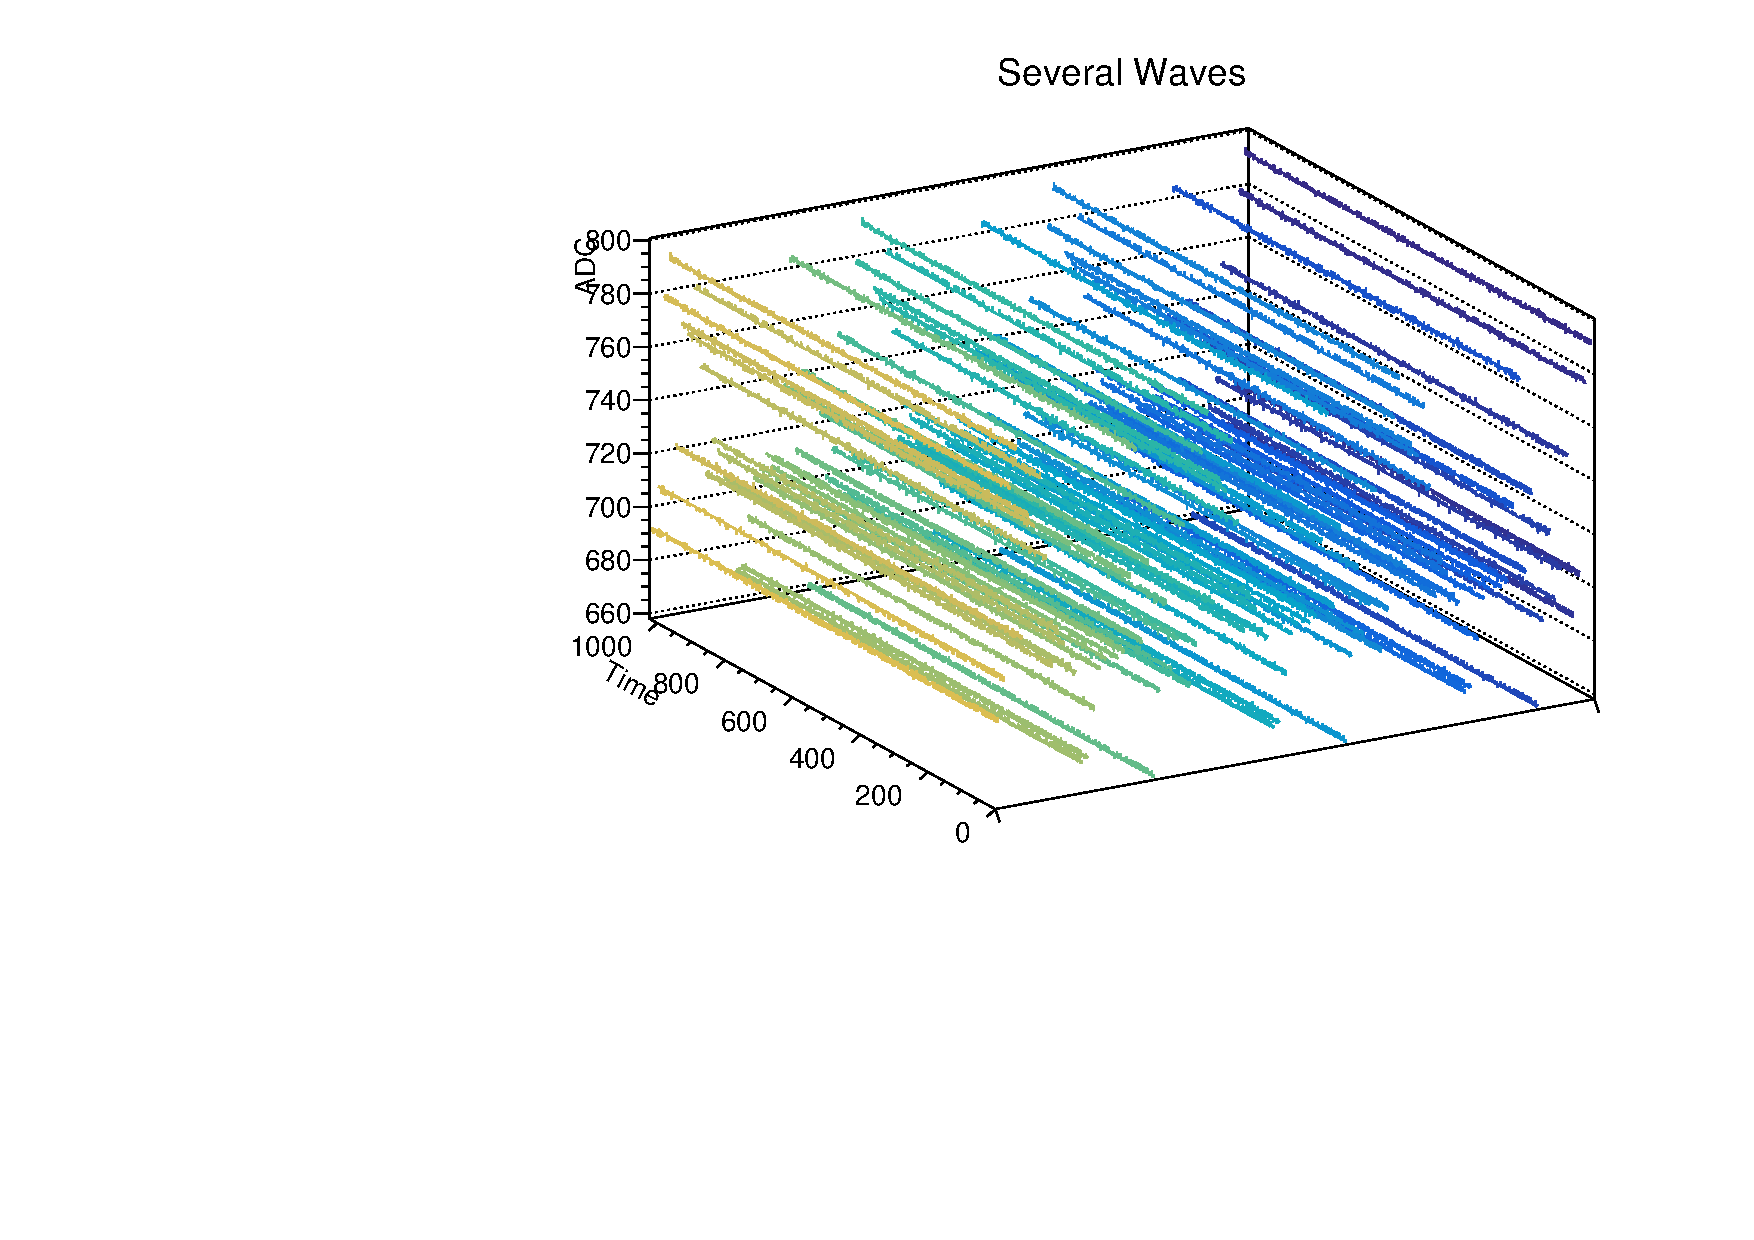
\includegraphics[width=\textwidth]{240115_12_wfeb_SeveralWaves.pdf}
    \caption{ADC[1:0] 连接FEB测试基线}
    \label{fig:adc12_wfeb}
  \end{subfigure}
  \hfill
  \begin{subfigure}[b]{0.45\textwidth}
    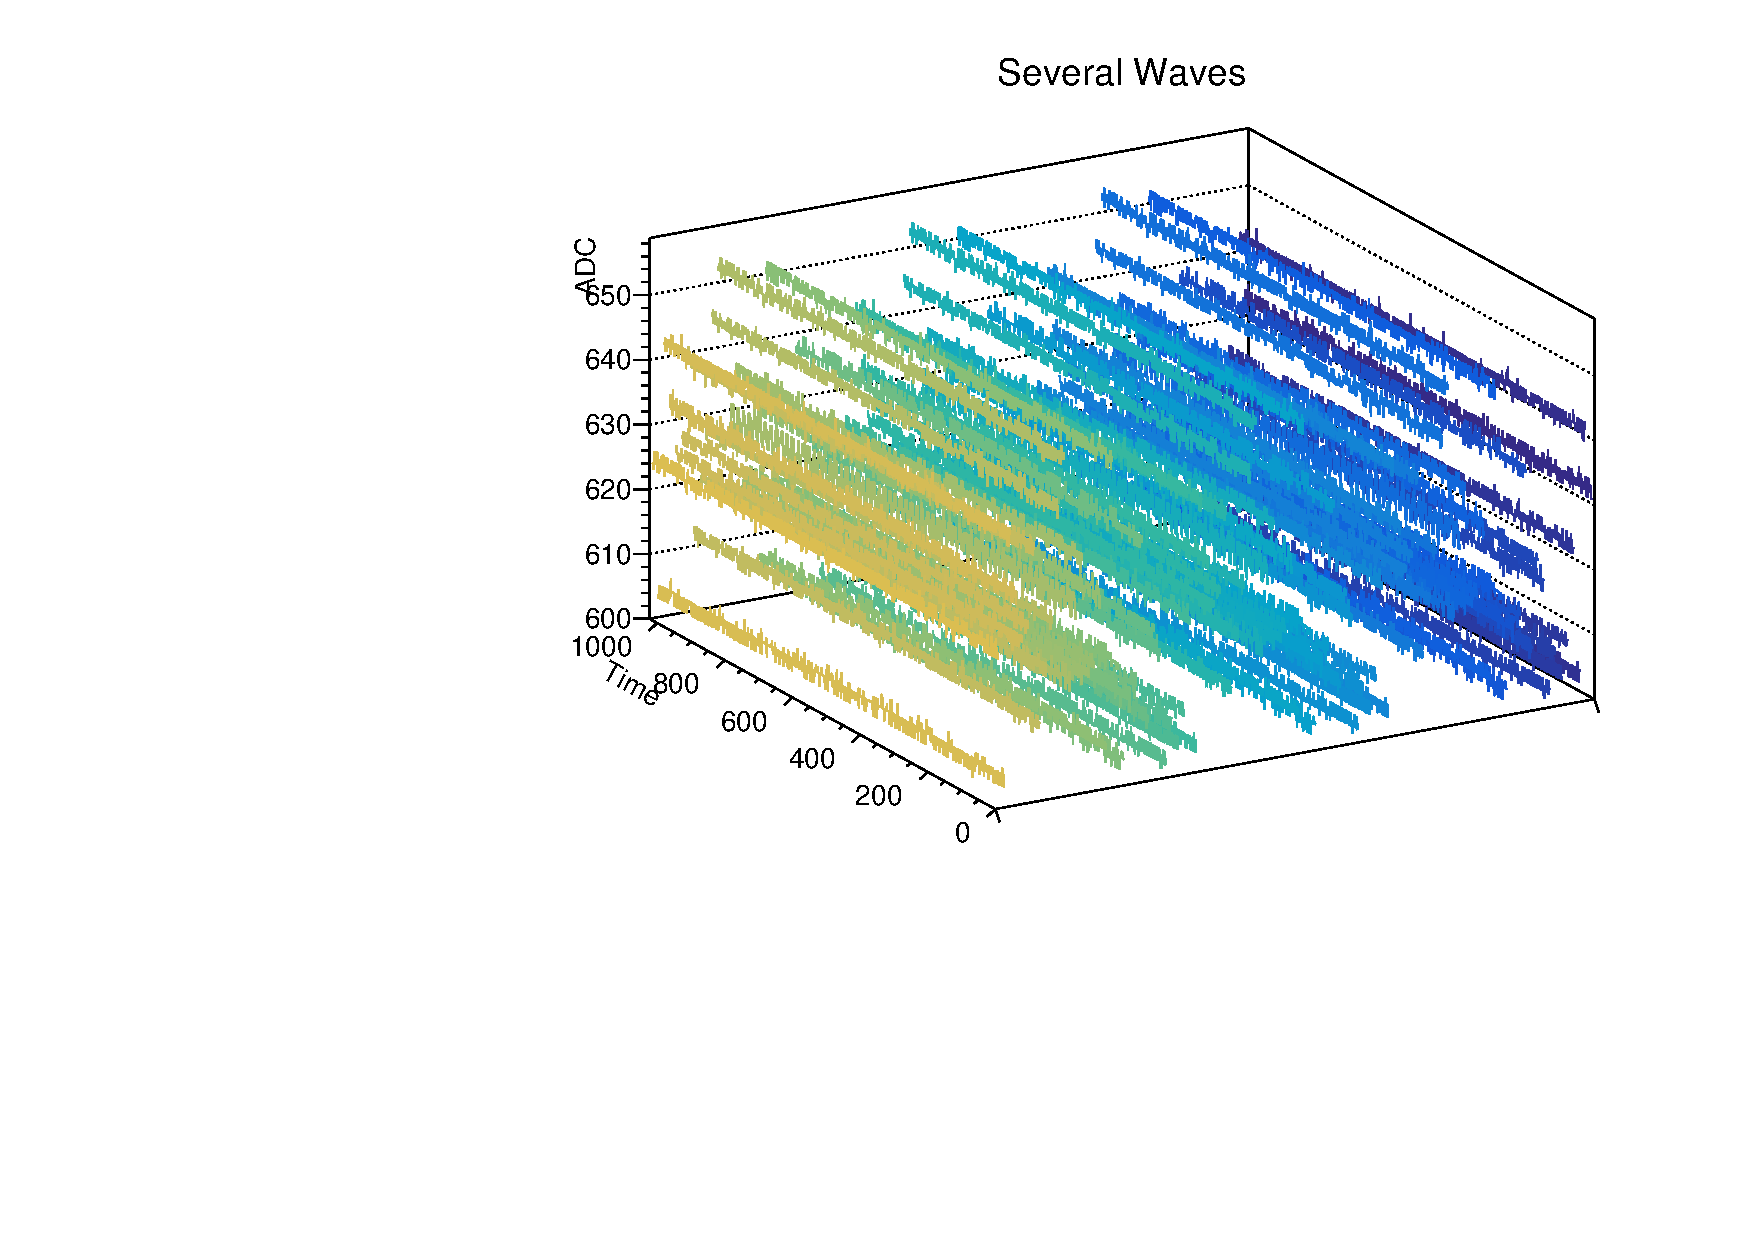
\includegraphics[width=\textwidth]{240115_34_wfeb_SeveralWaves.pdf}
    \caption{ADC[3:2] 连接FEB测试基线}
    \label{fig:adc34_wfeb2}
  \end{subfigure}
  \caption{ADC 连接FEB测试基线}
  \label{fig:ADC_wfeb}
\end{figure}

\section{FEB Map}
  \begin{longtable}{|c|c|c|c|c|c|c|c|c|c|c|c|}
    \hline
    \multicolumn{6}{|l|}{正:} & \multicolumn{6}{l|}{反:} \\ \hline
    \endfirsthead
    
    \hline
    \multicolumn{6}{|l|}{正:} & \multicolumn{6}{l|}{反:} \\ \hline
    \endhead
    
    \hline
    \endfoot
    
    \hline
    \endlastfoot
    
    Y55 & Y57 & Y59 & Y56 & Y58 & A6  & A4  & X58 & X56 & X59 & X57 & X55 \\ \hline
    0   & 4   & 6   & 64  & 68  & 71  & 70  & 67  & 65  & 7   & 5   & 1   \\ \hline
    X53 & X51 & X49 & X54 & X52 & A5  & A7  & Y52 & Y54 & Y49 & Y51 & Y53 \\ \hline
    3   & 15  & 13  & 79  & 76  & 75  & 72  & 66  & 69  & 12  & 14  & 2   \\ \hline
        & Y43 & Y45 & Y47 & Y48 & Y50 & X50 & X48 & X47 & X45 & X43 &     \\ \hline
        & 22  & 10  & 8   & 73  & 78  & 77  & 74  & 9   & 11  & 23  &     \\ \hline
        & X41 & X39 & X37 & X46 & X44 & Y44 & Y46 & Y37 & Y39 & Y41 &     \\ \hline
        & 21  & 17  & 19  & 86  & 83  & 84  & 87  & 18  & 16  & 20  &     \\ \hline
        & Y33 & Y35 & Y38 & Y40 & Y42 & X42 & X40 & X38 & X35 & X33 &     \\ \hline
        & 28  & 30  & 80  & 82  & 85  & 95  & 92  & 81  & 31  & 29  &     \\ \hline
        & X31 & X29 & X36 & X34 & X32 & Y32 & Y34 & Y36 & Y29 & Y31 &     \\ \hline
        & 25  & 27  & 93  & 90  & 91  & 88  & 89  & 94  & 26  & 24  &     \\ \hline
        & Y25 & Y27 & Y26 & Y28 & Y30 & X30 & X28 & X26 & X27 & X25 &     \\ \hline
        & 38  & 36  & 96  & 100 & 103 & 102 & 99  & 97  & 37  & 39  &     \\ \hline
        & X23 & X21 & X24 & X22 & X20 & Y20 & Y22 & Y24 & Y21 & Y23 &     \\ \hline
        & 35  & 33  & 111 & 108 & 107 & 104 & 98  & 101 & 32  & 34  &     \\ \hline
        & Y15 & Y17 & Y19 & Y16 & Y18 & X18 & X16 & X19 & X17 & X15 &     \\ \hline
        & 46  & 44  & 40  & 105 & 110 & 109 & 106 & 41  & 45  & 47  &     \\ \hline
        & X13 & X11 & X9  & X14 & X12 & Y12 & Y14 & Y9  & Y11 & Y13 &     \\ \hline
        & 53  & 55  & 43  & 118 & 116 & 115 & 119 & 42  & 54  & 52  &     \\ \hline
    Y5  & Y7  & A3  & Y6  & Y8  & Y10 & X10 & X8  & X6  & A1  & X7  & X5  \\ \hline
    48  & 50  & 62  & 112 & 124 & 117 & 127 & 114 & 113 & 63  & 51  & 49  \\ \hline
    X3  & X1  & A0  & X4  & X2  & X0  & Y0  & Y2  & Y4  & A2  & Y1  & Y3  \\ \hline
    59  & 57  & 61  & 125 & 121 & 123 & 120 & 122 & 126 & 60  & 56  & 58  \\ \hline

\end{longtable}

\section{转接板 Map}
\begin{longtable}{|c|c|c|c|}
  \hline
  转接板通道 & FEB 通道 & 阳极板通道 & ADC 通道 \\ \hline
  \endfirsthead
  
  \hline
  转接板通道 & FEB 通道 & 阳极板通道 & ADC 通道 \\ \hline
  \endhead
  
  \hline
  \endfoot
  
  \hline
  \endlastfoot
  
  X0    & A1     & X30   & 63     \\ \hline
  X1    & X1     & X31   & 57     \\ \hline
  X2    & X3     & X32   & 59     \\ \hline
  X3    & X5     & X33   & 49     \\ \hline
  X4    & X7     & X34   & 51     \\ \hline
  X5    & X9     & X35   & 43     \\ \hline
  X6    & X11    & X36   & 55     \\ \hline
  X7    & X13    & X37   & 53     \\ \hline
  X8    & X15    & X38   & 47     \\ \hline
  X9    & X17    & X39   & 45     \\ \hline
  X10   & X19    & X40   & 41     \\ \hline
  X11   & X21    & X41   & 33     \\ \hline
  X12   & X23    & X42   & 35     \\ \hline
  X13   & X25    & X43   & 39     \\ \hline
  X14   & X27    & X44   & 37     \\ \hline
  X15   & X29    & X45   & 27     \\ \hline
  X16   & X31    & X46   & 25     \\ \hline
  X17   & X33    & X47   & 29     \\ \hline
  X18   & X35    & X48   & 31     \\ \hline
  X19   & X37    & X49   & 19     \\ \hline
  X20   & X39    & X50   & 17     \\ \hline
  X21   & X41    & X51   & 21     \\ \hline
  X22   & X43    & X52   & 23     \\ \hline
  X23   & X45    & X53   & 11     \\ \hline
  X24   & X47    & X54   & 9      \\ \hline
  X25   & X49    & X55   & 13     \\ \hline
  X26   & X51    & X56   & 15     \\ \hline
  X27   & X53    & X57   & 3      \\ \hline
  X28   & X55    & X58   & 1      \\ \hline
  X29   & X57    & X59   & 5      \\ \hline
  X30   & A0     & Y30   & 61     \\ \hline
  X31   & X0     & Y31   & 123    \\ \hline
  X32   & X2     & Y32   & 121    \\ \hline
  X33   & X4     & Y33   & 125    \\ \hline
  X34   & X6     & Y34   & 113    \\ \hline
  X35   & X8     & Y35   & 114    \\ \hline
  X36   & X10    & Y36   & 127    \\ \hline
  X37   & X12    & Y37   & 116    \\ \hline
  X38   & X14    & Y38   & 118    \\ \hline
  X39   & X16    & Y39   & 106    \\ \hline
  X40   & X18    & Y40   & 109    \\ \hline
  X41   & X20    & Y41   & 107    \\ \hline
  X42   & X22    & Y42   & 108    \\ \hline
  X43   & X24    & Y43   & 111    \\ \hline
  X44   & X26    & Y44   & 97     \\ \hline
  X45   & X28    & Y45   & 99     \\ \hline
  X46   & X30    & Y46   & 102    \\ \hline
  X47   & X32    & Y47   & 91     \\ \hline
  X48   & X34    & Y48   & 90     \\ \hline
  X49   & X36    & Y49   & 93     \\ \hline
  X50   & X38    & Y50   & 81     \\ \hline
  X51   & X40    & Y51   & 92     \\ \hline
  X52   & X42    & Y52   & 95     \\ \hline
  X53   & X44    & Y53   & 83     \\ \hline
  X54   & X46    & Y54   & 86     \\ \hline
  X55   & X48    & Y55   & 74     \\ \hline
  X56   & X50    & Y56   & 77     \\ \hline
  X57   & X52    & Y57   & 76     \\ \hline
  X58   & X54    & Y58   & 79     \\ \hline
  X59   & X56    & Y59   & 65     \\ \hline
  Y0    & Y59    & X60   & 6      \\ \hline
  Y1    & Y57    & X61   & 4      \\ \hline
  Y2    & Y55    & X62   & 0      \\ \hline
  Y3    & Y53    & X63   & 2      \\ \hline
  Y4    & Y51    & X64   & 14     \\ \hline
  Y5    & Y49    & X65   & 12     \\ \hline
  Y6    & Y47    & X66   & 8      \\ \hline
  Y7    & Y45    & X67   & 10     \\ \hline
  Y8    & Y43    & X68   & 22     \\ \hline
  Y9    & Y41    & X69   & 20     \\ \hline
  Y10   & Y39    & X70   & 16     \\ \hline
  Y11   & Y37    & X71   & 18     \\ \hline
  Y12   & Y35    & X72   & 30     \\ \hline
  Y13   & Y33    & X73   & 28     \\ \hline
  Y14   & Y31    & X74   & 24     \\ \hline
  Y15   & Y29    & X75   & 26     \\ \hline
  Y16   & Y27    & X76   & 36     \\ \hline
  Y17   & Y25    & X77   & 38     \\ \hline
  Y18   & Y23    & X78   & 34     \\ \hline
  Y19   & Y21    & X79   & 32     \\ \hline
  Y20   & Y19    & X80   & 40     \\ \hline
  Y21   & Y17    & X81   & 44     \\ \hline
  Y22   & Y15    & X82   & 46     \\ \hline
  Y23   & Y13    & X83   & 52     \\ \hline
  Y24   & Y11    & X84   & 54     \\ \hline
  Y25   & Y9     & X85   & 42     \\ \hline
  Y26   & Y7     & X86   & 50     \\ \hline
  Y27   & Y5     & X87   & 48     \\ \hline
  Y28   & Y3     & X88   & 58     \\ \hline
  Y29   & Y1     & X89   & 56     \\ \hline
  Y30   & Y58    & Y61   & 68     \\ \hline
  Y31   & Y56    & Y62   & 64     \\ \hline
  Y32   & Y54    & Y63   & 69     \\ \hline
  Y33   & Y52    & Y64   & 66     \\ \hline
  Y34   & Y50    & Y65   & 78     \\ \hline
  Y35   & Y48    & Y66   & 73     \\ \hline
  Y36   & Y46    & Y67   & 87     \\ \hline
  Y37   & Y44    & Y68   & 84     \\ \hline
  Y38   & Y42    & Y69   & 85     \\ \hline
  Y39   & Y40    & Y70   & 82     \\ \hline
  Y40   & Y38    & Y71   & 80     \\ \hline
  Y41   & Y36    & Y72   & 94     \\ \hline
  Y42   & Y34    & Y73   & 89     \\ \hline
  Y43   & Y32    & Y74   & 88     \\ \hline
  Y44   & Y30    & Y75   & 103    \\ \hline
  Y45   & Y28    & Y76   & 100    \\ \hline
  Y46   & Y26    & Y77   & 96     \\ \hline
  Y47   & Y24    & Y78   & 101    \\ \hline
  Y48   & Y22    & Y79   & 98     \\ \hline
  Y49   & Y20    & Y80   & 104    \\ \hline
  Y50   & Y18    & Y81   & 110    \\ \hline
  Y51   & Y16    & Y82   & 105    \\ \hline
  Y52   & Y14    & Y83   & 119    \\ \hline
  Y53   & Y12    & Y84   & 115    \\ \hline
  Y54   & Y10    & Y85   & 117    \\ \hline
  Y55   & Y8     & Y86   & 124    \\ \hline
  Y56   & Y6     & Y87   & 112    \\ \hline
  Y57   & Y4     & Y88   & 126    \\ \hline
  Y58   & Y2     & Y89   & 122    \\ \hline
  Y59   & Y0     & A11   & 120    \\ \hline
  A3    & A6     & A3    & 71     \\ \hline
  A6    & X59    & A6    & 7      \\ \hline
  A9    & A7     & Y60   & 72     \\ \hline
  A12   & A5     & A12   & 75     \\ \hline
  
\end{longtable}

\section{TPC Map}
\subsection{大 TPC}
\subsubsection{按 ADC 通道}
\noindent
\resizebox{\textwidth}{!}{
\begin{tabular}{|c|c|c|c|c|c|c|c|}
  \hline
  ADC 通道 & TPC 通道 & ADC 通道 & TPC 通道 & ADC 通道 & TPC 通道 & ADC 通道 & TPC 通道 \\ \hline
  
  0      & Y04    & 32     & Y47    & 64     & Y05    & 96     & Y53    \\ \hline
  1      & X04    & 33     & X47    & 65     & X05    & 97     & X53    \\ \hline
  2      & Y06    & 34     & Y50    & 66     & Y08    & 98     & Y49    \\ \hline
  3      & X06    & 35     & X50    & 67     & X02    & 99     & A14    \\ \hline
  4      & Y03    & 36     & Y54    & 68     & Y02    & 100    & A15    \\ \hline
  5      & X03    & 37     & X54    & 69     & Y07    & 101    & Y51    \\ \hline
  6      & Y01    & 38     & Y52    & 70     & X00    & 102    & A10    \\ \hline
  7      & X01    & 39     & X52    & 71     & Y00    & 103    & Y42    \\ \hline
  8      & A03    & 40     & Y45    & 72     & A01    & 104    & Y48    \\ \hline
  9      & A02    & 41     & X45    & 73     & Y12    & 105    & Y43    \\ \hline
  10     & Y28    & 42     & Y22    & 74     & X12    & 106    & X43    \\ \hline
  11     & A08    & 43     & X22    & 75     & A00    & 107    & X48    \\ \hline
  12     & Y11    & 44     & Y44    & 76     & X08    & 108    & X49    \\ \hline
  13     & X11    & 45     & X44    & 77     & X10    & 109    & X46    \\ \hline
  14     & Y09    & 46     & A13    & 78     & Y10    & 110    & Y46    \\ \hline
  15     & X09    & 47     & A12    & 79     & X07    & 111    & X51    \\ \hline
  16     & Y35    & 48     & Y19    & 80     & Y34    & 112    & Y20    \\ \hline
  17     & X34    & 49     & X19    & 81     & X35    & 113    & X20    \\ \hline
  18     & Y36    & 50     & Y21    & 82     & Y32    & 114    & X23    \\ \hline
  19     & X36    & 51     & X21    & 83     & X30    & 115    & Y26    \\ \hline
  20     & Y33    & 52     & Y27    & 84     & Y29    & 116    & X26    \\ \hline
  21     & X32    & 53     & X27    & 85     & Y31    & 117    & Y25    \\ \hline
  22     & Y30    & 54     & Y24    & 86     & X28    & 118    & A06    \\ \hline
  23     & X29    & 55     & X24    & 87     & A09    & 119    & A07    \\ \hline
  24     & A11    & 56     & Y14    & 88     & Y41    & 120    & Y15    \\ \hline
  25     & X42    & 57     & X14    & 89     & Y39    & 121    & X16    \\ \hline
  26     & Y55    & 58     & Y17    & 90     & X40    & 122    & Y16    \\ \hline
  27     & X55    & 59     & X17    & 91     & X41    & 123    & X15    \\ \hline
  28     & Y40    & 60     & Y13    & 92     & X33    & 124    & Y23    \\ \hline
  29     & X39    & 61     & X13    & 93     & X38    & 125    & X18    \\ \hline
  30     & Y38    & 62     & A05    & 94     & Y37    & 126    & Y18    \\ \hline
  31     & X37    & 63     & A04    & 95     & X31    & 127    & X25    \\ \hline
  
  \end{tabular}
}

\subsubsection{按 TPC 通道}
\noindent
\resizebox{\textwidth}{!}{
\begin{tabular}{|c|c|c|c|c|c|c|c|c|c|}
  \hline
  TPC 通道 & ADC 通道 & TPC 通道 & ADC 通道 & TPC 通道 & ADC 通道 & TPC 通道 & ADC 通道 & TPC 通道 & ADC 通道 \\ \hline
  
  A00    & 75     & X00    & 70     & X28    & 86     & Y00    & 71     & Y28    & 10     \\ \hline
  A01    & 72     & X01    & 7      & X29    & 23     & Y01    & 6      & Y29    & 84     \\ \hline
  A02    & 9      & X02    & 67     & X30    & 83     & Y02    & 68     & Y30    & 22     \\ \hline
  A03    & 8      & X03    & 5      & X31    & 95     & Y03    & 4      & Y31    & 85     \\ \hline
  A04    & 63     & X04    & 1      & X32    & 21     & Y04    & 0      & Y32    & 82     \\ \hline
  A05    & 62     & X05    & 65     & X33    & 92     & Y05    & 64     & Y33    & 20     \\ \hline
  A06    & 118    & X06    & 3      & X34    & 17     & Y06    & 2      & Y34    & 80     \\ \hline
  A07    & 119    & X07    & 79     & X35    & 81     & Y07    & 69     & Y35    & 16     \\ \hline
  A08    & 11     & X08    & 76     & X36    & 19     & Y08    & 66     & Y36    & 18     \\ \hline
  A09    & 87     & X09    & 15     & X37    & 31     & Y09    & 14     & Y37    & 94     \\ \hline
  A10    & 102    & X10    & 77     & X38    & 93     & Y10    & 78     & Y38    & 30     \\ \hline
  A11    & 24     & X11    & 13     & X39    & 29     & Y11    & 12     & Y39    & 89     \\ \hline
  A12    & 47     & X12    & 74     & X40    & 90     & Y12    & 73     & Y40    & 28     \\ \hline
  A13    & 46     & X13    & 61     & X41    & 91     & Y13    & 60     & Y41    & 88     \\ \hline
  A14    & 99     & X14    & 57     & X42    & 25     & Y14    & 56     & Y42    & 103    \\ \hline
  A15    & 100    & X15    & 123    & X43    & 106    & Y15    & 120    & Y43    & 105    \\ \hline
          &        & X16    & 121    & X44    & 45     & Y16    & 122    & Y44    & 44     \\ \hline
          &        & X17    & 59     & X45    & 41     & Y17    & 58     & Y45    & 40     \\ \hline
          &        & X18    & 125    & X46    & 109    & Y18    & 126    & Y46    & 110    \\ \hline
          &        & X19    & 49     & X47    & 33     & Y19    & 48     & Y47    & 32     \\ \hline
          &        & X20    & 113    & X48    & 107    & Y20    & 112    & Y48    & 104    \\ \hline
          &        & X21    & 51     & X49    & 108    & Y21    & 50     & Y49    & 98     \\ \hline
          &        & X22    & 43     & X50    & 35     & Y22    & 42     & Y50    & 34     \\ \hline
          &        & X23    & 114    & X51    & 111    & Y23    & 124    & Y51    & 101    \\ \hline
          &        & X24    & 55     & X52    & 39     & Y24    & 54     & Y52    & 38     \\ \hline
          &        & X25    & 127    & X53    & 97     & Y25    & 117    & Y53    & 96     \\ \hline
          &        & X26    & 116    & X54    & 37     & Y26    & 115    & Y54    & 36     \\ \hline
          &        & X27    & 53     & X55    & 27     & Y27    & 52     & Y55    & 26     \\ \hline
  
  \end{tabular}
}

\subsection{小 TPC}
\subsubsection{按 ADC 通道}
\noindent
\resizebox{\textwidth}{!}{
\begin{tabular}{|c|c|c|c|c|c|c|c|}
  \hline
  ADC 通道 & TPC 通道 & ADC 通道 & TPC 通道 & ADC 通道 & TPC 通道 & ADC 通道 & TPC 通道 \\ \hline
  
  0      & Y55    & 32     & Y21    & 64     & Y56    & 96     & Y26    \\ \hline
  1      & X55    & 33     & X21    & 65     & X56    & 97     & X26    \\ \hline
  2      & Y53    & 34     & Y23    & 66     & Y52    & 98     & Y22    \\ \hline
  3      & X53    & 35     & X23    & 67     & X58    & 99     & X28    \\ \hline
  4      & Y57    & 36     & Y27    & 68     & Y58    & 100    & Y28    \\ \hline
  5      & X57    & 37     & X27    & 69     & Y54    & 101    & Y24    \\ \hline
  6      & Y59    & 38     & Y25    & 70     & A04    & 102    & X30    \\ \hline
  7      & X59    & 39     & X25    & 71     & A06    & 103    & Y30    \\ \hline
  8      & Y47    & 40     & Y19    & 72     & A07    & 104    & Y20    \\ \hline
  9      & X47    & 41     & X19    & 73     & Y48    & 105    & Y16    \\ \hline
  10     & Y45    & 42     & Y09    & 74     & X48    & 106    & X16    \\ \hline
  11     & X45    & 43     & X09    & 75     & A05    & 107    & X20    \\ \hline
  12     & Y49    & 44     & Y17    & 76     & X52    & 108    & X22    \\ \hline
  13     & X49    & 45     & X17    & 77     & X50    & 109    & X18    \\ \hline
  14     & Y51    & 46     & Y15    & 78     & Y50    & 110    & Y18    \\ \hline
  15     & X51    & 47     & X15    & 79     & X54    & 111    & X24    \\ \hline
  16     & Y39    & 48     & Y05    & 80     & Y38    & 112    & Y06    \\ \hline
  17     & X39    & 49     & X05    & 81     & X38    & 113    & X06    \\ \hline
  18     & Y37    & 50     & Y07    & 82     & Y40    & 114    & X08    \\ \hline
  19     & X37    & 51     & X07    & 83     & X44    & 115    & Y12    \\ \hline
  20     & Y41    & 52     & Y13    & 84     & Y44    & 116    & X12    \\ \hline
  21     & X41    & 53     & X13    & 85     & Y42    & 117    & Y10    \\ \hline
  22     & Y43    & 54     & Y11    & 86     & X46    & 118    & X14    \\ \hline
  23     & X43    & 55     & X11    & 87     & Y46    & 119    & Y14    \\ \hline
  24     & Y31    & 56     & Y01    & 88     & Y32    & 120    & Y00    \\ \hline
  25     & X31    & 57     & X01    & 89     & Y34    & 121    & X02    \\ \hline
  26     & Y29    & 58     & Y03    & 90     & X34    & 122    & Y02    \\ \hline
  27     & X29    & 59     & X03    & 91     & X32    & 123    & X00    \\ \hline
  28     & Y33    & 60     & A02    & 92     & X40    & 124    & Y08    \\ \hline
  29     & X33    & 61     & A00    & 93     & X36    & 125    & X04    \\ \hline
  30     & Y35    & 62     & A03    & 94     & Y36    & 126    & Y04    \\ \hline
  31     & X35    & 63     & A01    & 95     & X42    & 127    & X10    \\ \hline
  
  \end{tabular}
}

\subsubsection{按 TPC 通道}
\noindent
\resizebox{\textwidth}{!}{
\begin{tabular}{|c|c|c|c|c|c|c|c|c|c|}
  \hline
  TPC 通道 & ADC 通道 & TPC 通道 & ADC 通道 & TPC 通道 & ADC 通道 & TPC 通道 & ADC 通道 & TPC 通道 & ADC 通道 \\ \hline
  
  A0     & 61     & X00    & 123    & X30    & 102    & Y00    & 120    & Y30    & 103    \\ \hline
  A1     & 63     & X01    & 57     & X31    & 25     & Y01    & 56     & Y31    & 24     \\ \hline
  A2     & 60     & X02    & 121    & X32    & 91     & Y02    & 122    & Y32    & 88     \\ \hline
  A3     & 62     & X03    & 59     & X33    & 29     & Y03    & 58     & Y33    & 28     \\ \hline
  A4     & 70     & X04    & 125    & X34    & 90     & Y04    & 126    & Y34    & 89     \\ \hline
  A5     & 75     & X05    & 49     & X35    & 31     & Y05    & 48     & Y35    & 30     \\ \hline
  A6     & 71     & X06    & 113    & X36    & 93     & Y06    & 112    & Y36    & 94     \\ \hline
  A7     & 72     & X07    & 51     & X37    & 19     & Y07    & 50     & Y37    & 18     \\ \hline
          &        & X08    & 114    & X38    & 81     & Y08    & 124    & Y38    & 80     \\ \hline
          &        & X09    & 43     & X39    & 17     & Y09    & 42     & Y39    & 16     \\ \hline
          &        & X10    & 127    & X40    & 92     & Y10    & 117    & Y40    & 82     \\ \hline
          &        & X11    & 55     & X41    & 21     & Y11    & 54     & Y41    & 20     \\ \hline
          &        & X12    & 116    & X42    & 95     & Y12    & 115    & Y42    & 85     \\ \hline
          &        & X13    & 53     & X43    & 23     & Y13    & 52     & Y43    & 22     \\ \hline
          &        & X14    & 118    & X44    & 83     & Y14    & 119    & Y44    & 84     \\ \hline
          &        & X15    & 47     & X45    & 11     & Y15    & 46     & Y45    & 10     \\ \hline
          &        & X16    & 106    & X46    & 86     & Y16    & 105    & Y46    & 87     \\ \hline
          &        & X17    & 45     & X47    & 9      & Y17    & 44     & Y47    & 8      \\ \hline
          &        & X18    & 109    & X48    & 74     & Y18    & 110    & Y48    & 73     \\ \hline
          &        & X19    & 41     & X49    & 13     & Y19    & 40     & Y49    & 12     \\ \hline
          &        & X20    & 107    & X50    & 77     & Y20    & 104    & Y50    & 78     \\ \hline
          &        & X21    & 33     & X51    & 15     & Y21    & 32     & Y51    & 14     \\ \hline
          &        & X22    & 108    & X52    & 76     & Y22    & 98     & Y52    & 66     \\ \hline
          &        & X23    & 35     & X53    & 3      & Y23    & 34     & Y53    & 2      \\ \hline
          &        & X24    & 111    & X54    & 79     & Y24    & 101    & Y54    & 69     \\ \hline
          &        & X25    & 39     & X55    & 1      & Y25    & 38     & Y55    & 0      \\ \hline
          &        & X26    & 97     & X56    & 65     & Y26    & 96     & Y56    & 64     \\ \hline
          &        & X27    & 37     & X57    & 5      & Y27    & 36     & Y57    & 4      \\ \hline
          &        & X28    & 99     & X58    & 67     & Y28    & 100    & Y58    & 68     \\ \hline
          &        & X29    & 27     & X59    & 7      & Y29    & 26     & Y59    & 6      \\ \hline
  
  \end{tabular}
}